\section{SSH Protocol Overview}
\label{sec:overview}

\begin{figure*}[t]
  \centering

  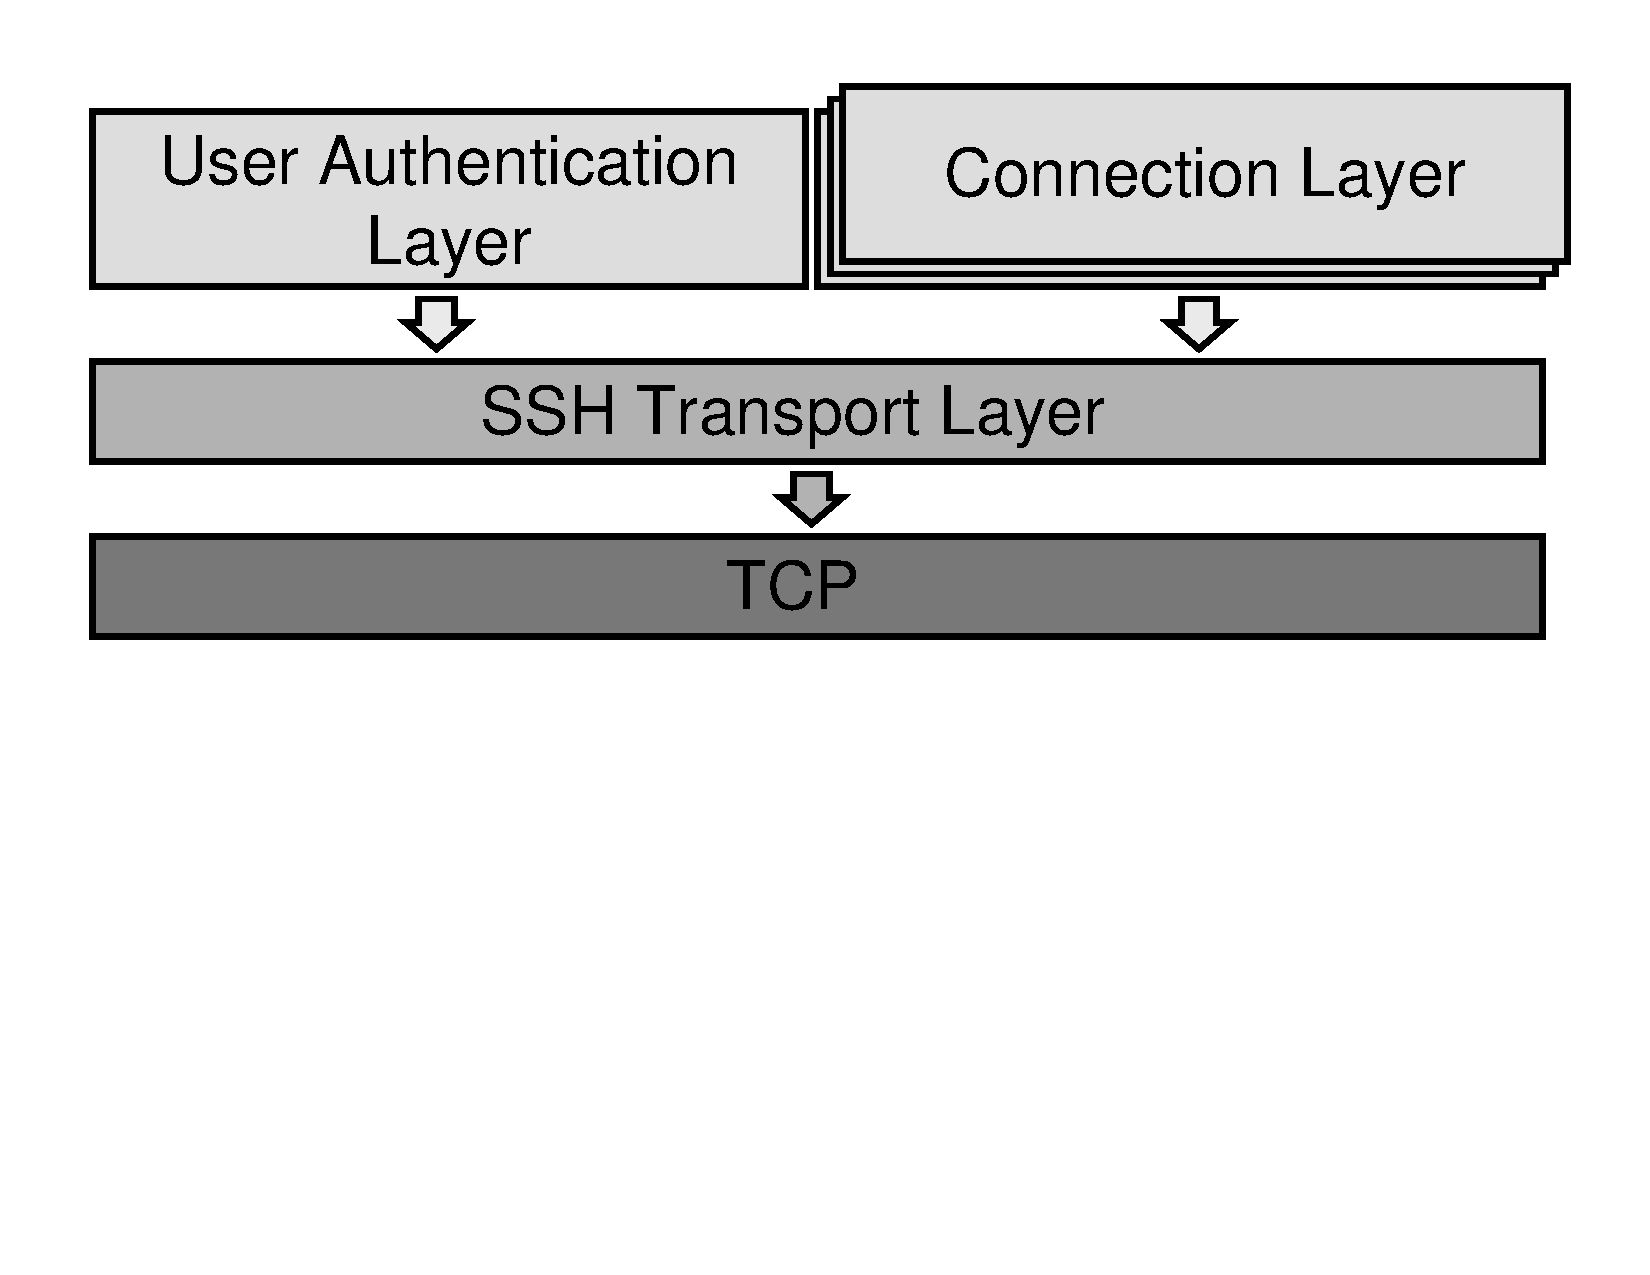
\includegraphics[width=0.9\textwidth,keepaspectratio=true]{sshlayer}
  \vspace{-13.5em}

  \caption{The hierarchy of layers within the SSH protocol.}
  \label{fig:ssh}
  \vspace{-1.5em}
\end{figure*}

The SSH protocol enables secure network services, including remote
login and traffic tunneling, over insecure networks such as the
Internet~\cite{rfc4251}. The functionality of the protocol is
partitioned into three layers, with each layer defined in terms of
messages from the layer beneath it. This hierarchy is depicted in
Figure~\ref{fig:ssh}; each layer plays a distinct role~\cite{rfc4251}:
\begin{itemize}
\item The \emph{transport layer} provides privacy, integrity, and
  server authentication for the user authentication protocols, as
  well as the application connection protocols, running on top of
  it. In short, it provides the layers above it with a plaintext
  interface for sending encrypted packets reliably over the network.
\item The \emph{user authentication layer} authenticates the client
  to the server. In keeping with the modular design of the protocol,
  this layer is extensible to a number of authentication
  mechanisms. The specification for this layer includes public key,
  password, and host-based authentication
  sub-protocols~\cite{rfc4252}. However, the majority of deployments
  use password-based authentication for its convenience and
  simplicity.
\item The \emph{connection layer} multiplexes many distinct
  communication channels over the SSH transport layer. Several channel
  types have been defined for various applications, including terminal
  shell channels for remote login, and traffic forwarding channels for
  encrypted tunnels.
\end{itemize}
A typical SSH session proceeds by working through these layers in
sequence: first, the SSH transport layer is established, after which
the user is able to securely authenticate to the server, and finally
the application-specific connections are initiated over the transport
layer.

\paragraph{Session Initialization:}

To establish the SSH transport layer, the server and client must
\textit{(1)} perform a key exchange to establish a shared secret that
is used to encrypt future communications, and \textit{(2)} validate
the server's key, to prevent a man-in-the-middle attack. The SSH
specification includes a single Diffie-Hellman group for key
exchange~\cite{rfc4251}, although later proposals have extended this
layer to allow new Diffie-Hellman groups to be added as
needed~\cite{rfc4419}. As described in Section~\ref{sec:intro}, the
host's key is validated by querying the user. Thus, this layer is
responsible for the vulnerability described in
Section~\ref{sec:intro}.

\paragraph{User Authentication:}

When the SSH transport layer has been established, the client and
server have a secure channel over which they can communicate, and the
server has supposedly been authenticated to the client. However, most
applications require the client to authenticate to the server. The
user authentication layer handles this in an extensible way, by
defining a set of messages that can be used to relay general
authentication data. The specification describes several mechanisms
for authentication, including the username/password method familiar to
all users of SSH, as well as public key-based
authentication~\cite{rfc4252}. However, as long as the server and
client software can agree on an authentication method, it is
straightforward to extend this layer to use new mechanisms that
provide better security. For example, Yang and Shieh proposed the use
of smart cards for
authentication~\cite{DBLP:journals/compsec/YangS99}, which has
subsequently been implemented in at least one SSH software
package~\cite{opensc}. Our proposed protocol fits into the SSH
protocol in this layer.

When password authentication is used, the protocol proceeds as
follows (depicted in Figure~\ref{fig:auth}):
\begin{enumerate}
\item The client sends to the server a message of type
  \texttt{SSH\_MSG\_USERAUTH\_REQUEST}, containing the username and
  password given by the user.
\item Based on the contents of the
  \texttt{SSH\_MSG\_USERAUTH\_REQUEST}, the server responds to the
  client in one of two ways:
  \begin{itemize}
    \item If password authentication is disallowed, or
      the username/password combination supplied is incorrect, then
      the server responds with an \\ \texttt{SSH\_MSG\_USERAUTH\_FAILURE}
      message.
    \item If password authentication is allowed, and the
      username/pass\-word combination is valid, then the server responds
      with an \\ \texttt{SSH\_MSG\_USERAUTH\_SUCCESS} message.
  \end{itemize}
\item If the server sends \texttt{SSH\_MSG\_USERAUTH\_SUCCESS}, then
  the client has successfully authenticated and may begin requesting
  services. Otherwise, the protocol terminates.
\end{enumerate}

\begin{figure*}[t]
  \centering

  \begin{tabular}{|rcl|}
    \hline
    \underline{Client} & & \underline{Server} \\
    $(U,P)$: username &&\\ and password &
    $\xrightarrow{\mathrm{\texttt{SSH\_MSG\_USERAUTH\_REQUEST}}(U,P)}$
    & \\
    & & \textbf{Check:} \\ && (1) Passwords supported \\ && (2) Credentials
    correct \\
    \textit{Success} & $\xleftarrow{\mathrm{\texttt{SSH\_MSG\_USERAUTH\_SUCCESS}}}$ & If yes \\
    \textit{Terminate} & $\xleftarrow{\mathrm{\texttt{SSH\_MSG\_USERAUTH\_FAILURE}}}$ &
    If no \\
    \hline
  \end{tabular}

  \caption{The SSH user authentication sub-protocol.}
  \label{fig:auth}
  \vspace{-1.5em}
\end{figure*}

%% \paragraph{Strong Mutual Authentication with SFE}

%% We propose to address the shortcomings of the current SSH protocol,
%% which arise due to poor authentication of the server in the
%% initialization of the SSH transport layer, by introducing a mechanism
%% for strong \emph{mutual authentication} in the user authentication
%% layer. Our protocol uses secure function evaluation (SFE) to compare
%% the hash of the client's password, stored on the server, with a hash
%% computed from the password provided by the client at authentication
%% time. If the comparison reveals that the two values are equal, then it
%% must be the case that the entity acting as the server actually
%% possesses a hash of the client's password, giving strong evidence for
%% the authenticity of the server. If not, then either the client or
%% server is an impersonator and the protocol can terminate, not having
%% leaked any additional information to the adversary other than the
%% outcome of the authentication attempt~\cite{yao82}. We discuss this
%% protocol in greater detail in Section~\ref{sec:protocol}.

\begin{figure*}
  \centering

  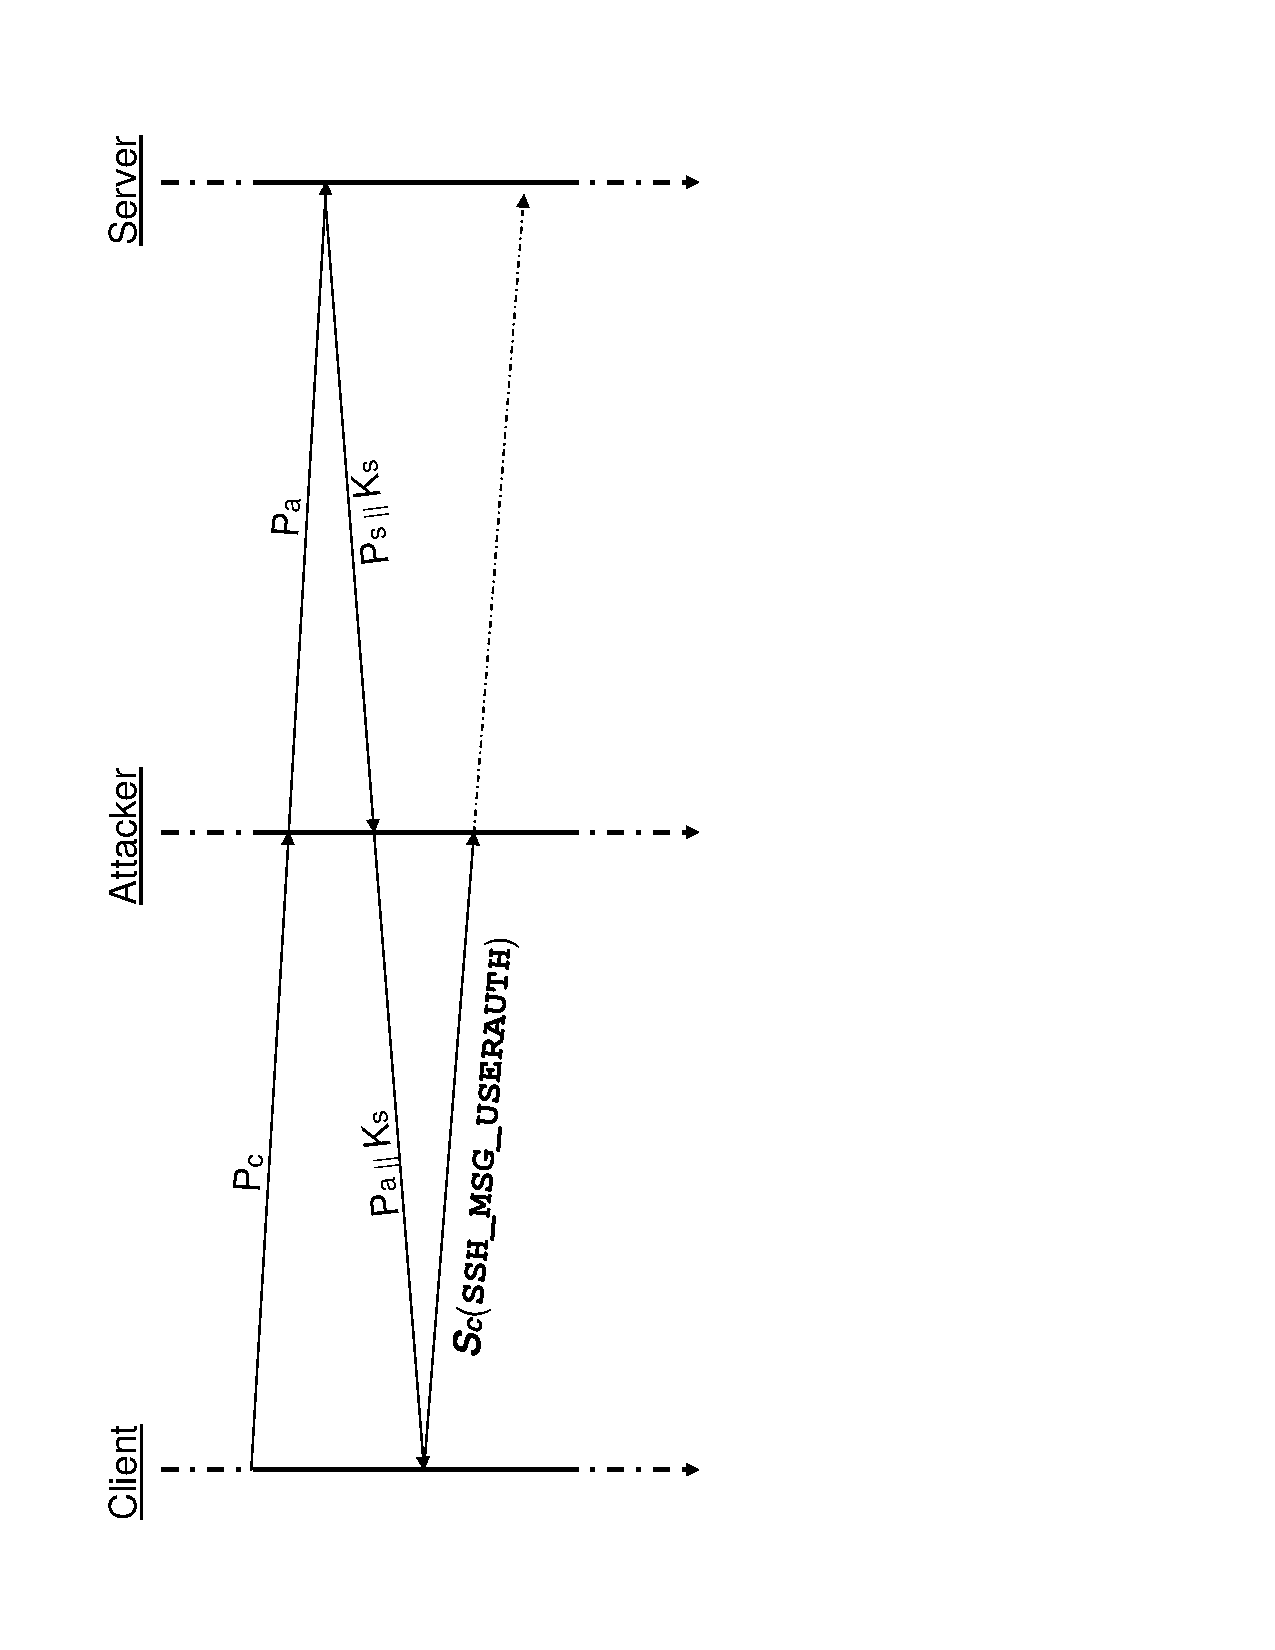
\includegraphics[height=\textwidth,keepaspectratio=true,angle=-90]{mitm}
  \vspace{-12em}

  \caption{Man-in-the-middle attack on the SSH authentication protocol
  using Diffie-Hellman key exchange as described in the SSH-2.0
  specification. Using this attack, an adversary can learn the
  client's password, eavesdrop on all communications between client
  and server, and impersonate the server.}
  \label{fig:mitm}
  % \vspace{-2em}
\end{figure*}


\subsection{Man-in-the-middle attack on conventional SSH password authentication}  
\label{subsec:ssh-mitm}
When SSH password authentication is used, the client and server first
negotiate an encrypted tunnel, over which the client sends the
password for verification.  If an attacker was somehow able to
eavesdrop on this encrypted tunnel, the password itself would be
revealed to the attacker, who would then be able to impersonate
the client at will.  A man-in-the-middle attack on the encrypted
tunnel, if succesful, would allow such a password interception.
To prevent such an attack, SSH relies on \emph{host
keys}~\cite{rfc4252} to authenticate the server. However, host keys
alone do not entirely solve the problem, as it is necessary to
authenticate each server key when a session is initiated. Under
certain circumstances, an attacker may still be able to mount a
successful attack. Figure~\ref{fig:mitm} depicts this situation when
the Diffie-Hellman key exchange is used:
\begin{enumerate}
  \item After the client and server agree on a key exchange protocol,
    the client attempts to send the public exponentiated integer $P_c$
    to the client.
  \item The attacker intercepts $P_c$, replaces it with a value
    known to him, $P_a$, and sends it to the server.
  \item The server sends his public integer, along with a host key
  that is supposed to prove his identity: $P_s \parallel K_s$.
  \item The attacker intercepts $P_s \parallel K_s$ and sends $P_a
  \parallel K_a$ to the server.
  \item Using the exchanged public keys, the attacker constructs
    separate shared secrets $S_c$ and $S_s$ with the client and
    server, to be used for further communications.
  \item The client's software hashes the key that it receives, $K_a$,
    and checks a local keystore to see if the hash is recognized. If
    the client does not have the real servers's public key $K_a$ in his
    keystore, then the client software asks the user to verify the
    server key's authenticity:
    \begin{verbatim}[fontsize=\small,frame=single]
The authenticity of host 'server (1.2.3.4)' can't be 
established. RSA key fingerprint is 
3f:76:22:43:c2:03:b9:71:b0:31:ce:87:37:45:cb:02.
Are you sure you want to continue connecting (yes/no)?
    \end{verbatim}
  On the other hand, even if the user knows the correct server key,
  he may assume the key has changed for a non-malicious reason,
  such as a software upgrade, and allow the connection to proceed.
  \item The user validates the authenticity of the key based on its
    hexadecimal fingerprint, thereby mistakenly asserting that the
    attacker is the authentic server.
  \item The client attempts to send $S_c$(\texttt{SSH\_MSG\_USERAUTH})
    to the server, containing login credentials encrypted with the
    shared secret $S_c$. In this case, the credentials consist of a
    username and password.
  \item The attacker receives $S_c$(\texttt{SSH\_MSG\_USERAUTH}), and
    is able to decrypt it to read the password in clear text.
\end{enumerate}
Critical to the success of this attack is that the user validates the
authenticity of the attacker's public key as the server's, in step
\textit{(7)}, \emph{an action which we assert is highly probable}. Any
OpenSSH user is familiar with the message displayed in step
\textit{(6)} -- according to the SSH protocol RFC, the fingerprint
``\ldots can easily be verified by using telephone or other external
communication channels.''~\cite{rfc4251} Not surprisingly, recent
research has indicated that one can expect the average user to simply
\emph{click through} this dialog without going to such
trouble~\cite{adams-usability}, thus accepting the attacker's key;
this undermines the very purpose of presenting host key fingerprints
to the user. Although the designers of the SSH protocol were aware of
this problem when they released the specification, they assumed that
widespread future PKI deployment would make it
unimportant~\cite{rfc4251}.
